%!TEX program = lualatex
\documentclass[border=0mm,11pt]{standalone}
%\usepackage{color}
%\usepackage{tikz}
\usepackage[T1]{fontenc}
\usepackage[sc]{mathpazo}
\usepackage{tikz-feynman}
\tikzfeynmanset{compat=1.1.0}


\begin{document}

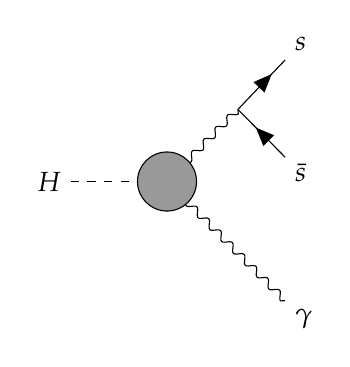
\begin{tikzpicture}[]
    \begin{feynman}[every blob={/tikz/fill=gray!80,/tikz/inner sep=0pt}]
    \vertex (h) {$H$};
    \vertex [right=of h, xshift=-0.0cm, yshift=-0.0cm] (cent);
    \vertex [right=of cent, xshift=-0.6cm, yshift=0.915cm] (pre-b);
    \vertex [right=of cent, xshift=0.0cm, yshift=1.75cm] (b) {$s$};
    \vertex [right=of cent, xshift=0.0cm, yshift=0.11cm] (e) {$\bar{s}$};
    \vertex [right=of cent, xshift=0.0cm, yshift=-1.75cm] (f) {$\gamma$};
    
    \diagram* {
    (h) -- [scalar] (cent),
    (b) -- [with reversed arrow=0.55] (pre-b) -- [with reversed arrow=0.65] (e),
    (cent) -- [photon] (pre-b),
    (cent) -- [photon] (f),
    };
    \node [blob] at (cent) {};
    \end{feynman}
\end{tikzpicture}

\end{document}